\chapter{Wymagania i narzędzia}
\label{ch:wymagania-i-narzedzia}

\section{Wymagania funkcjonalne i niefunkcjonalne}
\subsection{Wymagania funkcjonalne}

Wymagania funkcjonalne systemu stanowią kluczową część projektu, definiując precyzyjnie zachowania, funkcje i operacje, których oczekuje się od systemu w~celu zaspokojenia potrzeb użytkowników. Poprzez ich klarowne określenie możliwe jest wyznaczenie ram projektowych oraz stworzenie fundamentu dla późniejszego projektowania i implementacji systemu:

\begin{itemize}
	\item Możliwość zalogowania przy pomocy konta Spotify:
	\begin{itemize}
		\item Możliwość założenia sesji
		\item Możliwość przeglądania założonych sesji
		\item Możliwość usuwania sesji
		\item Możliwość moderacji sesji:
			\begin{itemize}
				\item Ograniczenie liczby utworów, które może dodać gość 
				\item Ograniczenie gatunków muzyki i autorów, które mogą być dodane
				\item Zmiana kolejności utworów w kolejce 
				\item Nadanie priorytetu danemu gościowi, aby jego utwory pojawiały się wcześniej 
				\item Zablokowanie możliwości dodawania utworów danemu gościowi 
				\item Ograniczenie liczby gości, którzy mogą dołączyć do sesji 
				\item Ograniczenie maksymalnej długości utworów, które mogą być dodane
				\item Możliwość włączenia funkcji głosowania, aby pomijać obecny utwór oraz ustawienia liczby głosów wymaganych do zatwierdzenia głosowania 
			\end{itemize}
			
		\item Możliwość sterowania odtwarzaczem:
		\begin{itemize}
			\item Zatrzymanie lub wznowienie odtwarzania
			\item Zmiana głośności odtwarzania
			\item Pomijanie lub cofanie do poprzedniego utworu 
		\end{itemize}
	\end{itemize} 
	
	\item Możliwość dołączenia do sesji jako gość: 
	\begin{itemize}
		\item Dołączenie do sesji odbywa się przez zeskanowanie kodu QR bądź użycie kodu dostępu 
		\item Możliwość ustawienia pseudonimu widocznego w sesji 
		\item Możliwość wyszukania utworów z bazy Spotify 
		\item Możliwość dodania wyszukanego utworu do kolejki
	\end{itemize}
	
	\item Możliwość zapisania playlisty z danej sesji przez wszystkich użytkowników w sesji
	\item Aplikacja podpowiada kolejne utwory bazując na ostatnio dodanych 
\end{itemize}

\subsection{Wymagania niefunkcjonalne}
Wymagania niefunkcjonalne to kluczowe kryteria, które określają cechy systemu, takie jak wydajność, bezpieczeństwo czy skalowalność, nie będącymi bezpośrednio związane z~jego funkcjonalnością. Definiują one granice, w których system musi działać, obejmując aspekty takie jak wydajność, dostępność czy też wymagania dotyczące interfejsu użytkownika:
\begin{itemize}
	\item Aplikacja internetowa kompatybilna z różnymi urządzeniami mobilnymi, oraz różnymi systemami operacyjnymi
	\item Zabezpieczenie systemu przed nieautoryzowanym dostępem
	\item Użytkownicy nie mają możliwości ingerencji w konto Spotify właściciela sesji za wyjątkiem przewidzianej funkcji (dodawanie utworów do kolejki odtwarzania)
	\item Aplikacja ma posiadać prosty oraz intuicyjny interfejs użytkownika z osobnymi panelami dla gościa oraz właściciela sesji umożliwiający realizację funkcjonalności aplikacji
	\item Zapewnienie możliwości dalszej rozbudowy systemu oraz aktualizacji
	\item System jest zależny od API serwisu Spotify
	\item System jest zgodny z warunkami użytkowania serwisu Spotify \cite{bib:spotify_terms}
	\item System posiada bazę danych SQL, w której przetrzymywane są informacje o~użytkownikach, sesjach etc. 
	\item Aplikacja jest ograniczona przez limit zapytań nałożony przez Spotify (w przypadku osiągnięcia takiego limitu użytkownik będzie zmuszony odczekać pewien czas przed kontynuacją użytkowania aplikacji)
	\item System jest w stanie obsłużyć wielu użytkowników oraz wiele sesji na raz.
\end{itemize}

\section{Przypadki użycia}
Zgodnie z rys. \ref{fig:use-case}, aby skorzystać z systemu należy się najpierw zalogować jednym z~dwóch sposobów. Gdy intencją użytkownika jest zakładanie oraz zarządzanie sesją należy użyć do logowania swojego konta Spotify. Następnie użytkownik ma możliwość założenia nowej sesji i ustawienia jej zasad, sterowanie odtwarzaczem muzyki lub dołączenie do jednej z istniejących już sesji lub usunięcie jej. Pozostali użytkownicy (goście) logują się używając kodu dostępu przez co dołączają do sesji. Wszyscy użytkownicy należący do sesji mogą wyszukiwać utwory oraz dodawać wybrane do kolejki odtwarzania.
\begin{figure}[h]
\centering
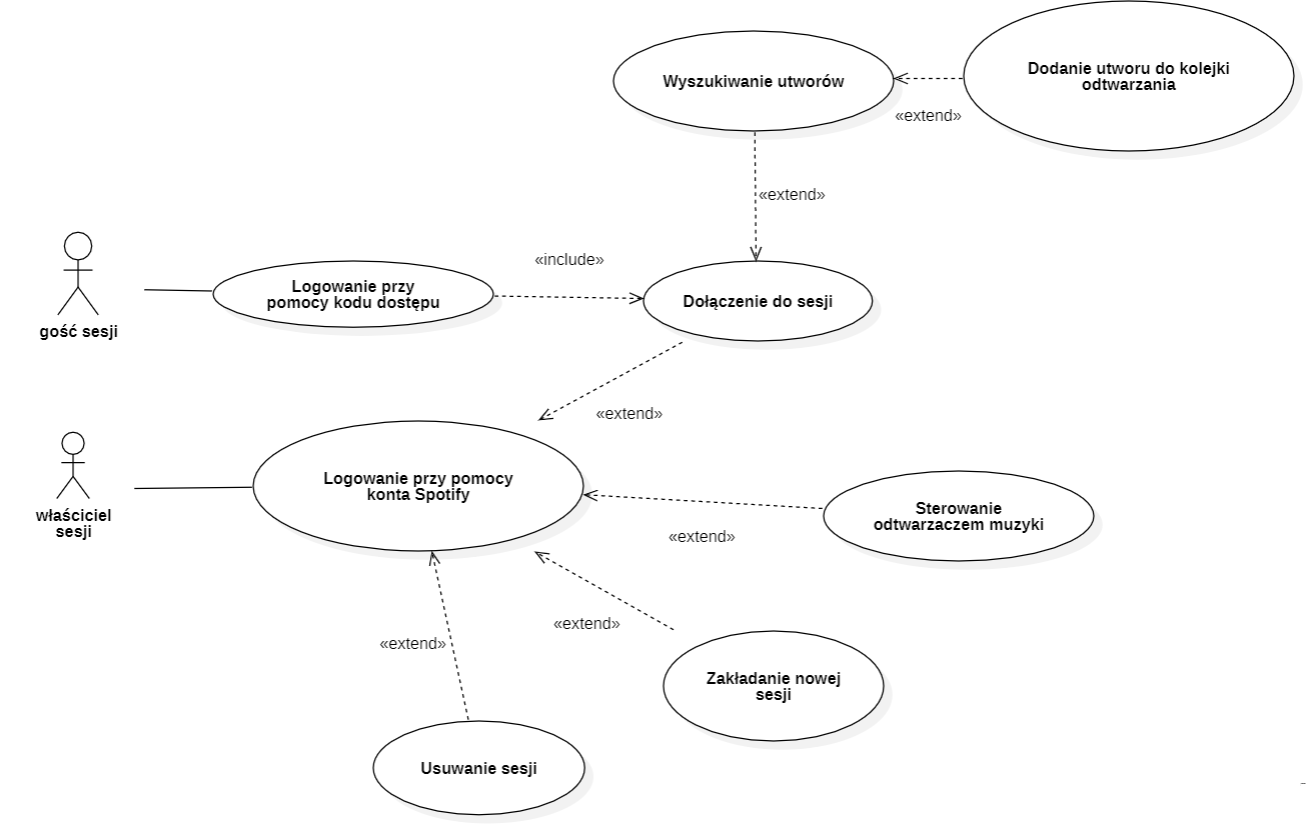
\includegraphics[width=0.95\textwidth]{./graf/przypadki_uzycia.PNG}
\caption{Przypadki użycia systemu}
\label{fig:use-case}
\end{figure}



\section{Opis narzędzi}

\subsection{Technologie serwera aplikacji (warstwa usług)}
Warunkami doboru technologii do wykonania części pracy działającej na serwerze była przede wszystkim uniwersalność oraz bezpieczeństwo aplikacji. Z tego powodu wybrany został język Java, który uruchamiany jest na wirtualnej maszynie (ang. \english{Java Virtual Machine}, JVM) wprowadzającej dodatkową warstwę abstrakcji między kodem Java a sprzętem komputerowym. JVM posiada wiele mechanizmów bezpieczeństwa (np. izolacja kodu czy automatyczne zarządzanie pamięcią) oraz umożliwia bezproblemowe uruchamianie programu na różnych platformach \cite{bib:java_virtual_machine}. Dużym atutem jest także ogromna społeczność programistów oraz bogaty ekosystem narzędzi oraz bibliotek, które można wykorzystać w projektach, co znacznie przyspiesza proces tworzenia oprogramowania.

Wraz z językiem Java użyta została platforma programistyczna Spring Boot \cite{bib:spring_boot}, która znacznie ułatwia tworzenie aplikacji serwerowych, przez dostarczanie gotowych rozwiązań oraz domyślne konfiguracje. Dużym atutem jest także modularność - architektura opiera się na mikro-serwisach, które pozwalają na dzielenie aplikacji na mniejsze części, co znacznie ułatwia skalowanie oraz dalszy rozwój aplikacji. Obecnie do tworzenia oprogramowania w Javie, Spring Boot jest najczęściej wybieraną platformą programistyczną \cite{bib:spring_market_analysis}.

Aby usprawnić implementację warstwy bazy danych, użyty został moduł Spring Data JPA \cite{bib:spring_jpa}, który umożliwia pominięcie pisania dużych ilości kodu SQL, ponieważ podstawowe operacje CRUD są automatycznie generowane. Programista tworząc klasę, która będzie odpowiedzialna za komunikację z bazą danych musi jedynie zaimplementować odpowiedni interfejs programistyczny. Dodatkowo umożliwia generowanie bardziej skomplikowanych zapytań wykorzystując do tego nazwę metody oraz mechanizm refleksji, w praktyce oznacza to, że pisanie jakiegokolwiek kodu SQL może się okazać zbędne. Spring Data JPA jest bardzo elastyczny i umożliwia korzystanie z różnych systemów bazodanowych oraz zapewnia automatyczne mapowanie obiektów Javy na tabele w~relacyjnej bazie danych (ang. \english{Object-Relational Mapping}, ORM).

Komunikacja z API Spotify została uproszczona przez użycie gotowego klienta \cite{bib:spotify_client_java}, który jest narzędziem programistycznym wprowadzającym dodatkową warstwę abstrakcji ukrywającą szczegóły komunikacji z zewnętrznym API, co ułatwia tworzenie oprogramowania i pozwala programiście skupić się na logice aplikacji.

\subsection{Technologie interfejsu użytkownika (warstwa prezentacji)}
Kluczowym aspektem w tworzeniu interfejsu użytkownika jest jego przejrzystość, intuicyjność oraz w jaki sposób aplikacja będzie zarządzać stanem. Dodatkowo, zgodnie z~założeniami projektu, system powinien być przystosowany do działania na urządzeniach mobilnych. Aby spełnić te wymogi do implementacji użyty został język TypeScript wraz z platformą programistyczną Angular \cite{bib:angular}, której głównym przeznaczeniem jest tworzenie jednostronicowych aplikacji internetowych (ang. \english{Single Page Application}, SPA). Dużą zaletą takiego rozwiązania jest pozbycie się konieczności przeładowywania zawartości strony w trakcie użytkowania aplikacji - zwiększa to interaktywność oraz efektywniej wykorzystuje zasoby. Dodatkowym atutem jest modularność, co minimalizuje powtarzalność tworzonego kodu oraz asynchroniczność wywoływania zapytań, która pozwala użytkownikowi na dalsze korzystanie z aplikacji pomimo oczekiwania na odpowiedź serwera. Angular zapewnia także wsparcie dla przeglądarek internetowych na urządzeniach mobilnych.

Dodatkowo w projekcie użyta została biblioteka Angular Materials \cite{bib:angular_materials}, która udostępnia gotowe szablony komponentów takich, jak wyskakujące okienka czy gotowe elementy formularzy. Pozwala to przyśpieszyć pracę nad tworzeniem oprogramowania.

\subsection{Baza danych (warstwa danych)}
Do realizacji warstwy danych użyty został system zarządzania bazami danych PostgreSQL. Dużą zaletą tego rozwiązania jest wysoka niezawodność zapewniona przez między innymi system kontroli spójności. Dodatkowym atutem jest skalowalność, która pozwala na zastosowanie tego rozwiązania zarówno w małych jak i w dużych systemach. 

\subsection{Platformy i usługi zewnętrzne}
Aby zapewnić spójność między warstwą prezentacji a warstwą usług wykorzystany został generator kodu \cite{bib:openapi_generator}, który na podstawie utworzonego przez programistę pliku opisującego powstające API (punkty końcowe, sposób autoryzacji, przyjmowane oraz zwracane wartości, opis obiektów uczestniczących w~wymianie między serwerem a~klientem itp.) generuje interfejsy programistyczne, obiekty modelu aplikacji oraz serwisy wykonujące zapytania w docelowym kodzie i wybranej technologii (w tym przypadku Java-Spring Boot oraz TypeScript-Angular), można powiedzieć że tworzony jest szkielet aplikacji pozbawiony logiki. Rolą programisty jest implementacja tych interfejsów oraz zastosowanie gotowych serwisów w odpowiednich miejscach zarówno po stronie klienta jak i serwera. Takie rozwiązanie ułatwia wprowadzanie zmian w wymianie klient-serwer oraz usprawnia tworzenie oprogramowania.

W projekcie użyta została platforma Docker \cite{bib:docker}, która umożliwia konteneryzację oprogramowania, co oznacza uruchomienie aplikacji z gotowego obrazu (program wraz z zależnościami takimi jak biblioteki, pliki konfiguracyjne etc.) na wirtualnej maszynie, z~którą można się komunikować oraz dowolnie zarządzać. Platforma wykorzystana była do symulacji serwera bazy danych.

\subsection{Środowisko deweloperskie}
Do implementacji oraz rozwoju omawianego systemu zostało użyte środowisko IntelliJ IDEA, zapewniające wsparcie dla języka Java oraz umożliwiające korzystanie z wtyczek oraz rozszerzeń, które znacznie ułatwiają pracę programisty. Interfejs użytkownika został utworzony przy pomocy Visual Studio Code, który wspiera składnię HTML, CSS oraz TypeScript.